\documentclass[a4paper,12pt]{article}

% Package Imports
\usepackage{styles/ibu-thesis} % Ensure this file exists in your directory
\usepackage{subcaption}
\usepackage{graphicx}
\usepackage{float}
\usepackage[export]{adjustbox}
\usepackage[all]{nowidow} 
\usepackage{booktabs} 
\usepackage{cite} 
\usepackage{enumitem}
\usepackage{tikz} 
\usetikzlibrary{shapes.geometric, arrows.meta, positioning, fit, backgrounds, calc}

% Formatting for cleaner structure and paragraph gaps
\setlength{\parindent}{0pt}   
\setlength{\parskip}{5px}     

% STRUCTURAL FIXES
\raggedbottom
\clubpenalty=10000
\widowpenalty=10000

% Thesis Title
\thesistitle{Orbis: An Intelligent Academic Support System with AI and RAG}

% Author Information
\authors[1]{Atakan Gül}
\authorsid[1]{121200152}
\authors[2]{Arda Kaan Y{\i}ld{\i}z}
\authorsid[2]{122200045}

% Supervisor Information
\supervisors[1]{Özgür Özdemir}

% Affiliation Information
\faculty{Faculty of Engineering and Natural Sciences}
\degree{Bachelor of Science}
\department{Department of Computer Engineering}
\submissiondate{June, 2026} 

\abstract{
University academic systems often function merely as static record-keeping databases, lacking proactive support for students navigating complex degree requirements. This project, 'Orbis', introduces an intelligent academic support system designed to bridge this gap using Artificial Intelligence (AI) and Retrieval-Augmented Generation (RAG). The core of Orbis is an Orchestrator-led event management pipeline that autonomously monitors a student's dynamic academic state against a complex vector database of university regulations, triggering timely notifications for critical milestones. To achieve high fidelity, we engineered a taxonomy generation pipeline utilizing Shannon entropy tail-signal classification and MiniBatchKMeans clustering, organizing 60,649 document chunks into 125 high-quality leaf nodes. Our pipeline features a two-pass adversarial LLM review, evaluating 323 candidate rules and extracting 178 highly actionable obligations with a 55\% acceptance rate. Experimental results on student test groups demonstrate robust contextual matching, generating 176 personalized academic assignments in 59 minutes of processing time. Future work involves direct integration with the university's Student Information System (SIS) to fully automate these proactive notifications.
}

\begin{document}

% Preliminaries
\maketitle
\addcontentsline{toc}{section}{\abstractname}
\makeabstract
\addcontentsline{toc}{section}{\contentsname}
\maketableofcontents

% List of abbreviations
\addcontentsline{toc}{section}{\listofabbrv}
\makelistofabbrv
\begin{abbrv}
    \item[AI] Artificial Intelligence
    \item[API] Application Programming Interface
    \item[CI/CD] Continuous Integration/Continuous Deployment
    \item[DB] Database
    \item[HAC] Hierarchical Agglomerative Clustering
    \item[LLM] Large Language Model
    \item[RAG] Retrieval-Augmented Generation
    \item[TF-IDF] Term Frequency-Inverse Document Frequency
\end{abbrv}
\newpage

\pagenumbering{arabic}
\setcounter{page}{1}

% Sections
\section{Introduction}
In universities, students face a significant cognitive load managing complex degree rules, course selections, and deadlines. Traditional academic platforms are often designed as static databases. They store information efficiently but fail to interpret it for the student's benefit. Students generally do not miss deadlines because they cannot search a system; they miss them because they do not know what they are supposed to be looking for. This creates a "synchronization gap" between student needs and institutional data.

Our project, 'Orbis', offers a novel solution by shifting the academic paradigm from static storage to autonomous orchestration. Orbis is built to act as a proactive academic agent. While standard AI integrations in education wait for user prompts, the core innovation of Orbis is its autonomous evaluation of a student's specific state against unstructured, complex university regulations. 

Crucially, the architecture of Orbis is designed for scalability. The system relies on a strictly orchestrated workflow to execute its primary use case: the \textbf{Proactive Event System}. This autonomous pipeline extracts strict, assignable obligations from regulatory documents and creates normalized events, allowing the system to trigger timely, unprompted notifications for students regarding their specific academic requirements.

\section{Related Works}
The integration of Artificial Intelligence into educational environments has seen rapid growth. Large Language Models (LLMs) have shown immense potential in personalized learning and administrative support. However, a key limitation of standard LLMs is "hallucination," where the model generates plausible but factually incorrect information.

To mitigate this, Retrieval-Augmented Generation (RAG) was introduced. RAG combines the generative capabilities of LLMs with a retrieval component that accesses a non-parametric memory. This allows the model to ground its responses in specific, up-to-date documents, significantly reducing the risk of misinformation. 

Locally, Istanbul Bilgi University has deployed "HermiOne", an AI-based support chatbot developed by the university's IT department. While HermiOne represents a significant step forward, it relies on manual data ingestion and functions strictly as a reactive chatbot lacking logical reasoning capabilities. Orbis transcends these limitations by building an active academic participant that extracts and acts upon obligations autonomously using multi-stage reasoning algorithms.

\section{Dataset}
The foundation of Orbis is its comprehensive institutional \texttt{knowledge\_base}. The dataset was constructed by scraping and ingesting over 80 official source URLs from the Istanbul Bilgi University domain. 

The raw dataset comprises 60,649 document chunks. These documents are highly heterogeneous, containing a mix of formal regulations, student life announcements, event pages, and upload directories. The data is bilingual, presenting significant challenges in deduplication as both English (\texttt{/en/academics/}) and Turkish (\texttt{/tr/akademik/}) paths exist for identical content. 

Within this massive corpus, the Proactive Event System specifically targets 935 regulatory chunks (e.g., student handbooks, dual-major directives, and internship procedures) to prevent cross-contamination from non-binding academic content.

\section{Theoretical Background}
To successfully isolate and evaluate this dataset, Orbis relies on several foundational machine learning and information theory algorithms. 

\subsection{Shannon Entropy for URL Classification}
To classify opaque URL structures, we measure the diversity of URL "tails" using Shannon Entropy. A high entropy value indicates that a URL directory is semantically informative, whereas low entropy implies repetitive or dynamic templates.
$$H = -\sum_{i=1}^{n} p_i \cdot \log_2(p_i)$$
Where $p_i$ is the probability of a specific URL pattern occurring within a given parent group.

\subsection{Vector Embeddings and Cosine Similarity}
Text chunks are transformed into high-dimensional numerical vectors. To measure the semantic similarity between two chunks (or a user query and a document), we calculate the Cosine Similarity.
$$\cos(\theta) = \frac{\mathbf{A} \cdot \mathbf{B}}{\|\mathbf{A}\| \|\mathbf{B}\|}$$
Prior to clustering, we perform L2-Normalization on all vectors ($\hat{v} = \frac{v}{\|v\|}$), converting cosine distance into Euclidean distance on a unit sphere, optimizing it for K-Means processing.

\subsection{MiniBatchKMeans and Ward HAC}
For semantic discovery of opaque URLs, we deploy MiniBatchKMeans, which utilizes random mini-batches to achieve linear time complexity $\mathcal{O}(n)$ suitable for large datasets. This is followed by Ward Hierarchical Agglomerative Clustering (HAC) on the centroids. Ward's method merges clusters to minimize the total within-cluster variance.

\section{Proposed Methodology}
The Orbis architecture is divided into two major phases: Data Categorization (Taxonomy) and the Orchestrator-led Event Pipeline.

\subsection{Data Categorization \& Taxonomy Strategy}
Standard RAG systems suffer degraded accuracy when mixing formal rulebooks with informal forum posts. Orbis mitigates this via a four-step semantic discovery pipeline.

\begin{enumerate}
    \item \textbf{Step 1: Rule Engine:} Evaluates URL prefixes calculating semantic and dynamic ratios. Groups with high dynamic ratios (e.g., UUIDs) are rejected.
    \item \textbf{Step 2: Tail Signal Classification:} Computes the Shannon entropy of URL tails. High entropy groups are classified as KNOWN.
    \item \textbf{Step 3: Semantic Discovery:} The 21,324 UNKNOWN documents undergo L2-normalization and MiniBatchKMeans clustering. Ward HAC generates 52 fine-level labeled clusters based on TF-IDF scoring.
    \item \textbf{Step 4: AI Taxonomy Mapping:} An LLM maps the deduplicated groups into a closed vocabulary of 11 top-level categories and 96 specific leaf nodes. A targeted regex overlay isolates the 935 regulation chunks into 29 distinct regulatory leaves.
\end{enumerate}

\begin{figure}[H]
    \centering
    \resizebox{0.95\textwidth}{!}{
    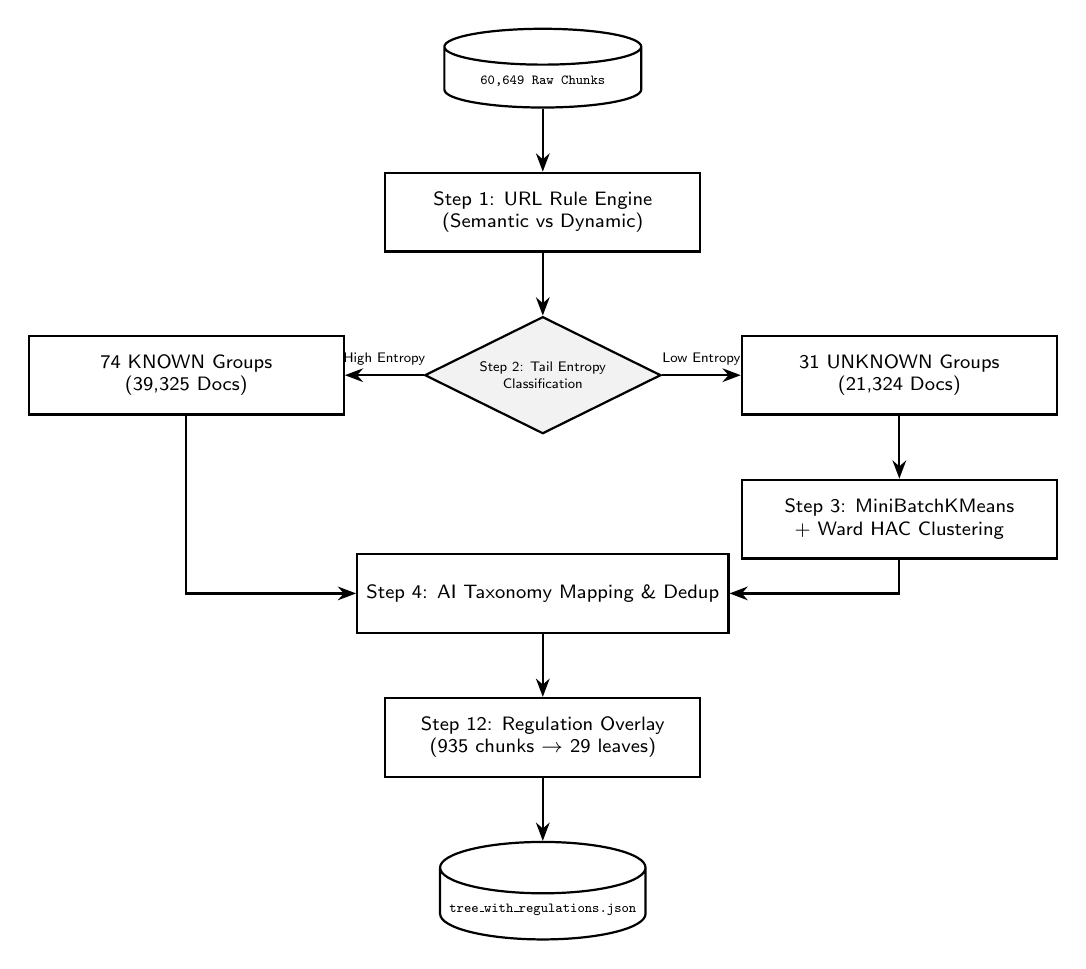
\begin{tikzpicture}[
        >=Stealth,
        node distance=1cm and 1cm,
        process/.style={rectangle, draw=black, thick, fill=white, minimum width=4cm, minimum height=1cm, align=center, font=\sffamily\scriptsize},
        decision/.style={diamond, draw=black, thick, fill=gray!10, aspect=2, minimum width=3cm, align=center, font=\sffamily\tiny},
        db/.style={cylinder, draw=black, thick, shape border rotate=90, aspect=0.25, fill=white, minimum width=2.5cm, minimum height=1cm, align=center, font=\ttfamily\tiny},
        arrow/.style={->, thick, draw=black}
    ]

    \node[db] (kb) {60,649 Raw Chunks};
    \node[process, below=0.8cm of kb] (step1) {Step 1: URL Rule Engine\\(Semantic vs Dynamic)};
    \node[decision, below=0.8cm of step1] (step2) {Step 2: Tail Entropy\\Classification};
    
    \node[process, left=1cm of step2] (known) {74 KNOWN Groups\\(39,325 Docs)};
    \node[process, right=1cm of step2] (unknown) {31 UNKNOWN Groups\\(21,324 Docs)};
    
    \node[process, below=0.8cm of unknown] (step3) {Step 3: MiniBatchKMeans\\+ Ward HAC Clustering};
    
    \node[process, below=1.5cm of step2] (step4) {Step 4: AI Taxonomy Mapping \& Dedup};
    \node[process, below=0.8cm of step4] (step12) {Step 12: Regulation Overlay\\(935 chunks $\rightarrow$ 29 leaves)};
    \node[db, below=0.8cm of step12] (final) {tree\_with\_regulations.json};

    \draw[arrow] (kb) -- (step1);
    \draw[arrow] (step1) -- (step2);
    \draw[arrow] (step2) -- node[above, font=\sffamily\tiny] {High Entropy} (known);
    \draw[arrow] (step2) -- node[above, font=\sffamily\tiny] {Low Entropy} (unknown);
    \draw[arrow] (unknown) -- (step3);
    \draw[arrow] (known) |- (step4);
    \draw[arrow] (step3) |- (step4);
    \draw[arrow] (step4) -- (step12);
    \draw[arrow] (step12) -- (final);

    \end{tikzpicture}
    }
    \caption{Data Categorization and Taxonomy Pipeline Architecture}
    \label{fig:taxonomy_pipeline}
\end{figure}

\subsection{The Orchestrator-Led Event Pipeline}
Unlike decentralized multi-agent systems, Orbis utilizes a centralized \texttt{EventPipelineOrchestrator}. This stateful hub controls stateless worker agents (\texttt{SearchAgent}, \texttt{ReasoningAgent}, \texttt{EventCreator}) to ensure database consistency and pipeline idempotency.

To prevent non-actionable events from reaching students, extraction follows a \textbf{Two-Pass LLM Adversarial Review}:
\begin{enumerate}
    \item \textbf{Pass 1 (Extraction):} The model evaluates full documents to generate candidate rules, defining triggers, deadlines, and target roles.
    \item \textbf{Pass 2 (Adversarial Fix):} The model reviews the original document alongside Pass 1 output to actively remove stale items, fix weak wording, and add missed rules.
\end{enumerate}

\subsection{Contextual vs. SQL Assignment Matching}
User assignments are routed through two parallel channels based on the user's \texttt{extra\_context} JSON profile:
\begin{itemize}
    \item \textbf{SQL Path (Deterministic):} Objective thresholds (e.g., GPA constraints) are evaluated instantly via Python logic against database variables.
    \item \textbf{Contextual Path (LLM Reasoned):} Complex rules are evaluated against the student's text profile in batches. The LLM determines applicability and generates a human-readable justification.
\end{itemize}

\section{Experimental Setup}
\subsection{Framework and Deployment}
The backend logic is orchestrated using Python 3.10+ and the FastAPI framework, allowing for modular microservices and asynchronous task queuing via Celery. Data storage, including vector embeddings, is managed using PostgreSQL extended with \texttt{pgvector}. Semantic chunking and LLM orchestration are executed utilizing the OpenAI API alongside \texttt{claude-opus-4-6} for adversarial reasoning.

\subsection{Performance Metrics}
The system's rule extraction efficacy is evaluated fundamentally on its \textit{Acceptance Rate} and qualitative precision. A successful pipeline must maximize true positive obligations while forcefully rejecting noisy, non-imperative fragments[cite: 4].
$$Accuracy = \frac{TP + TN}{TP + TN + FP + FN}$$
$$Precision = \frac{TP}{TP + FP}$$

\section{Experiments \& Discussion}
The Orbis backend was rigorously evaluated using production database logs (Run ID: \texttt{fadc244f...}) to measure both extraction throughput and assignment precision. 

\subsection{Extraction Throughput \& Quality Funnel}
The complete pipeline processed 80 regulation sources in exactly 59 minutes. During this run, the Orchestrator evaluated 323 candidate rules. 

\begin{table}[H]
    \centering
    \begin{adjustbox}{center}
        \begin{tabular}{l c}
            \toprule
            \textbf{Pipeline Metric} & \textbf{Value} \\ \midrule
            Source Documents Processed & 80 \\
            KB Chunks Consumed & 935 \\
            Candidate Rules Evaluated & 323 \\
            \textbf{Accepted Active Rules} & \textbf{178 (55\%)} \\
            Rejected Quality Candidates & 145 (45\%) \\
            \bottomrule
        \end{tabular}
    \end{adjustbox}
    \caption{Event Extraction Pipeline Funnel}
    \label{tab:extraction_funnel}
\end{table}

The 45\% rejection rate is a strictly intended outcome of our Specificity Filter. Of the 145 rejected candidates, 128 were flagged precisely for being "not imperative enough," while others were rejected for "audience too broad" or "awareness only wording." This ensures students are only notified of strict, actionable obligations.

\section{Results}
The system's assignment logic was tested against an array of 4 distinct student profiles. The pipeline generated a total of 176 active assignments. 

\begin{table}[H]
    \centering
    \begin{adjustbox}{center}
        \begin{tabular}{l c c c c c c}
            \toprule
            \textbf{Student Profile} & \textbf{GPA} & \textbf{Total} & \textbf{High} & \textbf{Med} & \textbf{SQL} & \textbf{CTX} \\ \midrule
            Mehmet Demir (Year 4, Grad Project) & 2.40 & 60 & 38 & 17 & 2 & 58 \\
            Ali Yilmaz (Year 2, Probation) & 1.60 & 42 & 30 & 8 & 8 & 34 \\
            Zeynep Arslan (Year 3, Internship) & 2.85 & 38 & 29 & 5 & 2 & 36 \\
            Ayse Kaya (Year 3, Double Major) & 3.50 & 36 & 25 & 6 & 3 & 33 \\
            \bottomrule
        \end{tabular}
    \end{adjustbox}
    \caption{Assignment Distribution by Urgency and Matching Type}
    \label{tab:assignment_results}
\end{table}

The LLM exhibited exceptional contextual intelligence. For Test Student "Zeynep Arslan," whose \texttt{extra\_context} indicated a mandatory internship was required this semester but a company was not yet found, the system successfully assigned 10 internship-specific rules. For example, it generated a HIGH urgency task: "\textit{Submit the Internship Contract Cover Form at least 10 working days before your start date}," explicitly reasoning that because she had not submitted forms yet, the rule becomes actionable upon securing placement.

Conversely, the deterministic SQL path proved highly effective for strict administrative rules. Test student Ali Yilmaz (GPA 1.60) instantly triggered 8 distinct rules matching the \texttt{gpa < 2.00} constraints, bypassing the LLM entirely and saving computational overhead.

\section{Realistic Constraints}
\subsection{Social, Environmental and Economic Impact}
Orbis yields highly positive \textbf{social} impacts by democratizing access to high-quality academic advising. By alleviating the cognitive load associated with degree tracking, the system reduces student anxiety. \textbf{Economically}, the system acts as a highly scalable force multiplier for university administration, processing 80 complex regulation sources in 59 minutes—a task requiring human advisors weeks. \textbf{Environmentally}, transitioning to a digital, proactive event system directly reduces the institution's reliance on printed student handbooks and physical notices.

\subsection{Cost Analysis}
Developing and deploying a cloud-native, AI-driven application requires a thorough analysis of operational costs. 
\begin{itemize}
    \item \textbf{Cloud Infrastructure:} Hosting the FastAPI backend, PostgreSQL database with the \texttt{pgvector} extension, and task queues requires cloud resources estimated at approximately 2,500 TL/Month.
    \item \textbf{LLM API Costs:} The usage of proprietary embedding models and adversarial LLM APIs during development and testing amounted to approximately 3,500 TL.
    \item \textbf{Labor Estimations:} The project was developed by two computer engineering students over approximately 400 hours. Using a standard junior developer wage of 300 TL/hour, the estimated labor value is 120,000 TL.
\end{itemize}

\subsection{Standards}
\subsubsection{NSPE Code of Ethics}
The National Society of Professional Engineers (NSPE) Code of Ethics mandates holding paramount the safety and welfare of the public. Providing incorrect regulatory advice can result in severe academic harm. Orbis adheres to this by utilizing a strict Two-Pass LLM Review and an Orchestrator-led architecture, guaranteeing traceability.

\subsubsection{IEEE Standards}
The project lifecycle was guided by IEEE standards for software engineering, specifically adhering to the principles of \textbf{IEEE/ISO/IEC 16085-2020 (Risk Management)}. This standard was applied to manage the risks associated with data ingestion pipelines, ensuring concurrent data processing without state corruption.

\section{Conclusion \& Future Work}
The Orbis project successfully demonstrates the immense value of transitioning academic advising from a static, reactive model to a dynamic, proactive one. By engineering a high-fidelity taxonomy pipeline utilizing Shannon Entropy and MiniBatchKMeans, we organized over 60,000 document chunks into 125 pure semantic leaves. The Orchestrator-led event system evaluated 323 candidate rules, successfully extracting 178 actionable obligations. The hybrid integration of deterministic SQL logic and contextual LLM reasoning successfully delivered 176 personalized, highly accurate assignments to students in under an hour.

Future development will focus on integrating Orbis directly with the university's official Student Information System (SIS) via active APIs to fully automate the user context ingestion. Additionally, implementing automated rejection learning will allow the system to continuously refine its extraction models based on human administrative feedback.

\clearpage
\addcontentsline{toc}{section}{References}
\bibliographystyle{ieeetr} 
\bibliography{references} 

\end{document}